\documentclass[a4paper,12pt]{article}
\usepackage[utf8]{inputenc}
\usepackage[polish]{babel}
\let\lll\undefined % do babelu, avoiding conflict
\usepackage{polski}
\selectlanguage{polish}
\usepackage[T1]{fontenc}
\frenchspacing
\usepackage{indentfirst}
\usepackage{multicol} %https://www.sharelatex.com/learn/Multiple_columns
\usepackage{float} % option locking floats: [H]


\usepackage{amssymb}
\usepackage{amsmath}
\usepackage{amsfonts}
 
\usepackage[pdftex,dvipsnames]{xcolor} %red, green, blue, yellow, cyan, magenta, black, white
%polskie tabelki
\usepackage[nottoc]{tocbibind}

% Kropki w liczebnikach porzadkowych
\usepackage{titlesec}
\titlelabel{\thetitle.\quad}


\setlength{\parskip}{0.3\baselineskip}%
% \setlength{\parindent}{0pt}%

%polskie przypisy
\usepackage{caption}
\captionsetup{labelsep=period}
\captionsetup{font=small,labelfont=bf,labelsep=period,justification=centering}
\addto\captionspolish{\renewcommand{\figurename}{Rys.}}
\addto\captionspolish{\renewcommand{\tablename}{Tab.}}
\addto\captionspolish{\renewcommand{\seename}{zob.}}

\usepackage{geometry}
 \geometry{
 a4paper,
 %total={170mm,247mm}, % 170 257 20 20
 left=20mm,
 right=20mm,
 top=20mm,
 bottom=25mm,
 }   
   


\usepackage{listings}
\definecolor{mygreen}{RGB}{28,172,0} % color values Red, Green, Blue
\definecolor{mylilas}{RGB}{170,55,241}
% \newcounter{listing}
% \newenvironment{listing}[1][]{
% \refstepcounter{listing}\par\medskip \textbf{Kod~\thelisting. #1} \rmfamily}{\medskip}

\lstset{language=Matlab,%
    %basicstyle=\color{red},
    breaklines=true,%
    morekeywords={matlab2tikz},
    keywordstyle=\color{blue},%
    morekeywords=[2]{1}, keywordstyle=[2]{\color{black}},
    identifierstyle=\color{black},%
    stringstyle=\color{mylilas},
    commentstyle=\color{mygreen},%
    showstringspaces=false,%without this there will be a symbol in the places where there is a space
    numbers=left,%
    numberstyle={\tiny \color{black}},% size of the numbers
    numbersep=9pt, % this defines how far the numbers are from the text
    emph=[1]{for,end,break},emphstyle=[1]\color{red}, %some words to emphasise
    %emph=[2]{word1,word2}, emphstyle=[2]{style},    
    basicstyle=\small\ttfamily,
    frame=single,
    float
}


% \usepackage{svg}
%SVG for the first time using inkscape: for i in *.svg; do inkscape -D -z --file=$i  --export-pdf="${i%.*}.pdf" --export-latex .; done




\usepackage{xargs}                      % Use more than one optional parameter in a new commands
%
\usepackage[colorinlistoftodos,prependcaption,textsize=tiny]{todonotes}
\newcommandx{\unsure}[2][1=]{\todo[linecolor=red,backgroundcolor=red!25,bordercolor=red,#1]{#2}}
\newcommandx{\change}[2][1=]{\todo[linecolor=blue,backgroundcolor=blue!25,bordercolor=blue,#1]{#2}}
% \newcommandx{\info}[2][1=]{\todo[linecolor=OliveGreen,backgroundcolor=OliveGreen!25,bordercolor=OliveGreen,#1]{#2}}
% \newcommandx{\improvement}[2][1=]{\todo[linecolor=Plum,backgroundcolor=Plum!25,bordercolor=Plum,#1]{#2}}
% \newcommandx{\thiswillnotshow}[2][1=]{\todo[disable,#1]{#2}}

% \missingfigure[figwidth=6cm]{Testing a long text string}


\usepackage[section]{placeins} %\FloatBarrier
% \usepackage{hyperref}
   
\usepackage{fancyhdr}
\setlength{\headheight}{38pt}
\pagestyle{fancy}

\lhead{Sprawozdanie z grantu rektorskiego koła SKIK 2017}     \rhead{\today\quad
\includegraphics[width=1.5cm]{logo_skik}}
\lfoot{}            \cfoot{}        \rfoot{strona \thepage/7}

\title{Projekt przedmiotu Sieci Neuronowe i Neurokomputery wydziału EiTI Politechniki Warszawskiej}
\author{Artur Dobrogowski}


\font\radikalwut=radikalwut at 36pt
% \newcommand{\radikalwut}{}

\begin{document}

%
\begin{titlepage}
    \centering
    {\scshape\Large {\radikalwut Politechnika Warszawska}\\\par Wydział Elektroniki i Technik Informacyjnych\\Instytut Radioelektroniki i Technik Multimedialnych \par}
    \vspace{1cm}
    {\huge\scshape\bfseries Sprawozdanie\\\par}
    {\scshape\Large z pracy naukowo-badawczej własnej\\ finansowanej z grantu rektorskiego za rok 2017\\\par}
%     {\Large Umowa numer XXX Y/????/????\\\par}
    \vspace{1cm}
    {\Large\bfseries Budowa mobilnej stacji naziemnej do odbioru danych APRS z balonów stratosferycznych\\\par}
    \vspace{1cm}
    {\Large\textsl {Studenckie Koło Inżynierii Kosmicznej}\par}
    \vfill
    Wykonawcy: \par
    {\small
    \begin{multicols}{2}

    \par Artur \textsc{Dobrogowski} 
    \par Michał \textsc{Kocon}
    \par Maciej \textsc{Trębiński}
    \par Krzysztof \textsc{Wasilewski}
    \end{multicols}
}
    Kierownik pracy:\par
    dr inż. Krzysztof \textsc{Kurek}

    \vfill

% Bottom of the page
    {\large \today\par}
\end{titlepage}

\tableofcontents

\section{Wprowadzenie}

\section{Cel projektu}

Celem projektu jest opracowanie mobilnej stacji do łączności radiowej z balonem ze szczególnym zwróceniem uwagi na pasma radioamatorskie. Stacja składa się z:
\begin{itemize}
    \item statywu z elektronicznie sterowanymi antenami przy pomocy silników krokowych umożliwiających zmianę orientacji anten w płaszczyźnie azymutu i elewacji,
    \item wzmacniacza sygnału przychodzącego z anteny,
    \item zestawu filtrów pasmowo przepustowych,
    \item radia programowalnego (SDR – Software Defined Radio) do przetworzenia sygnału (wykorzystane zostało radio będące na stanie Laboratorium Technologii Kosmicznych WEiTI), do którego stworzone zostało oprogramowanie umożliwiające odbiór sygnałów
\end{itemize}  

	Opracowana stacja pozwala na odbiór sygnałów w paśmie radioamatorskim: UHF 430 MHz (opcjonalnie w paśmie VHF 140 MHz). 
	Stworzone oprogramowanie do radia programowalnego SDR umożliwia odbiór pakietów APRS – automatycznego systemu powiadamiania o pozycji, który jest zwykle wykorzystywany do lokalizacji balonów w misjach. Wykorzystanie radia programowalnego SDR pozwoli w przyszłości na proste dostosowanie stacji do odbioru innych typów sygnałów (które mogą być przesyłane z balonu) tylko przez zmiany oprogramowania, bez konieczności zmian sprzętowych (jeśli transmisja będzie realizowana w obsługiwanym paśmie częstotliwości).

	Wynikiem prac jest między innymi oprogramowanie pozwalające na odbiór danych systemu APRS i danych podczas trwania misji, z wykorzystaniem radia programowalnego SDR.
	Gotowa stacja stanowi atrakcyjny obiekt zainteresowania do zaprezentowania np. w trakcie targów studenckich kół naukowych KONIK, co pomoże w popularyzacji tematyki związanej z systemami satelitarnymi.
	Wiedza i doświadczenie inżynierskie  zdobyte przez członków Koła w trakcie realizacji projektu pozwolą myśleć o wzięciu udziału w edukacyjnych projektach balonowych organizowanych pod patronatem Europejskiej Agencji Kosmicznej.

\section{Koncepcja mobilnej stacji naziemnej}

Zgodnie z planem projektu powstała stacja składająca się z:

\begin{itemize}
 \item dwu-częściowego rotora wraz ze sterownikiem, czujnikami położenia i kompasem,
 \item wykorzystanego radia programowalnego SDR z oprogramowaniem do dekodowania odbieranego sygnału,
 \item układu FPGA z możliwością realizacji własnego demodulatora na innym paśmie,
 \item układu zasilania składającego się z: 
    \begin{itemize}
    \item akumulatora samochodowego o pojemności 20Ah i napięciu 12 V,
    \item przetwornicy do napięcia 5V do zasilenia układów logicznych rotora,
    \item prostownikia do ładowania akumulatora,
    \item przetwornicy do napięcia zmiennego 230V ze standardowym gniazdkiem do zasilania ewentualnych peryferiów takich jak laptop,
    \end{itemize}
\end{itemize}

Ponieważ nie mamy wykształcenia w zakresie wykonywania konstrukcji mechanicznych to nasz projekt jest realizacją wysoce amatorską, ale funkcjonalną. Największym problemem był dobór odpowiednich przekładni do uzyskania niskich i precyzyjnych obrotów.

\begin{figure}
    \centering
    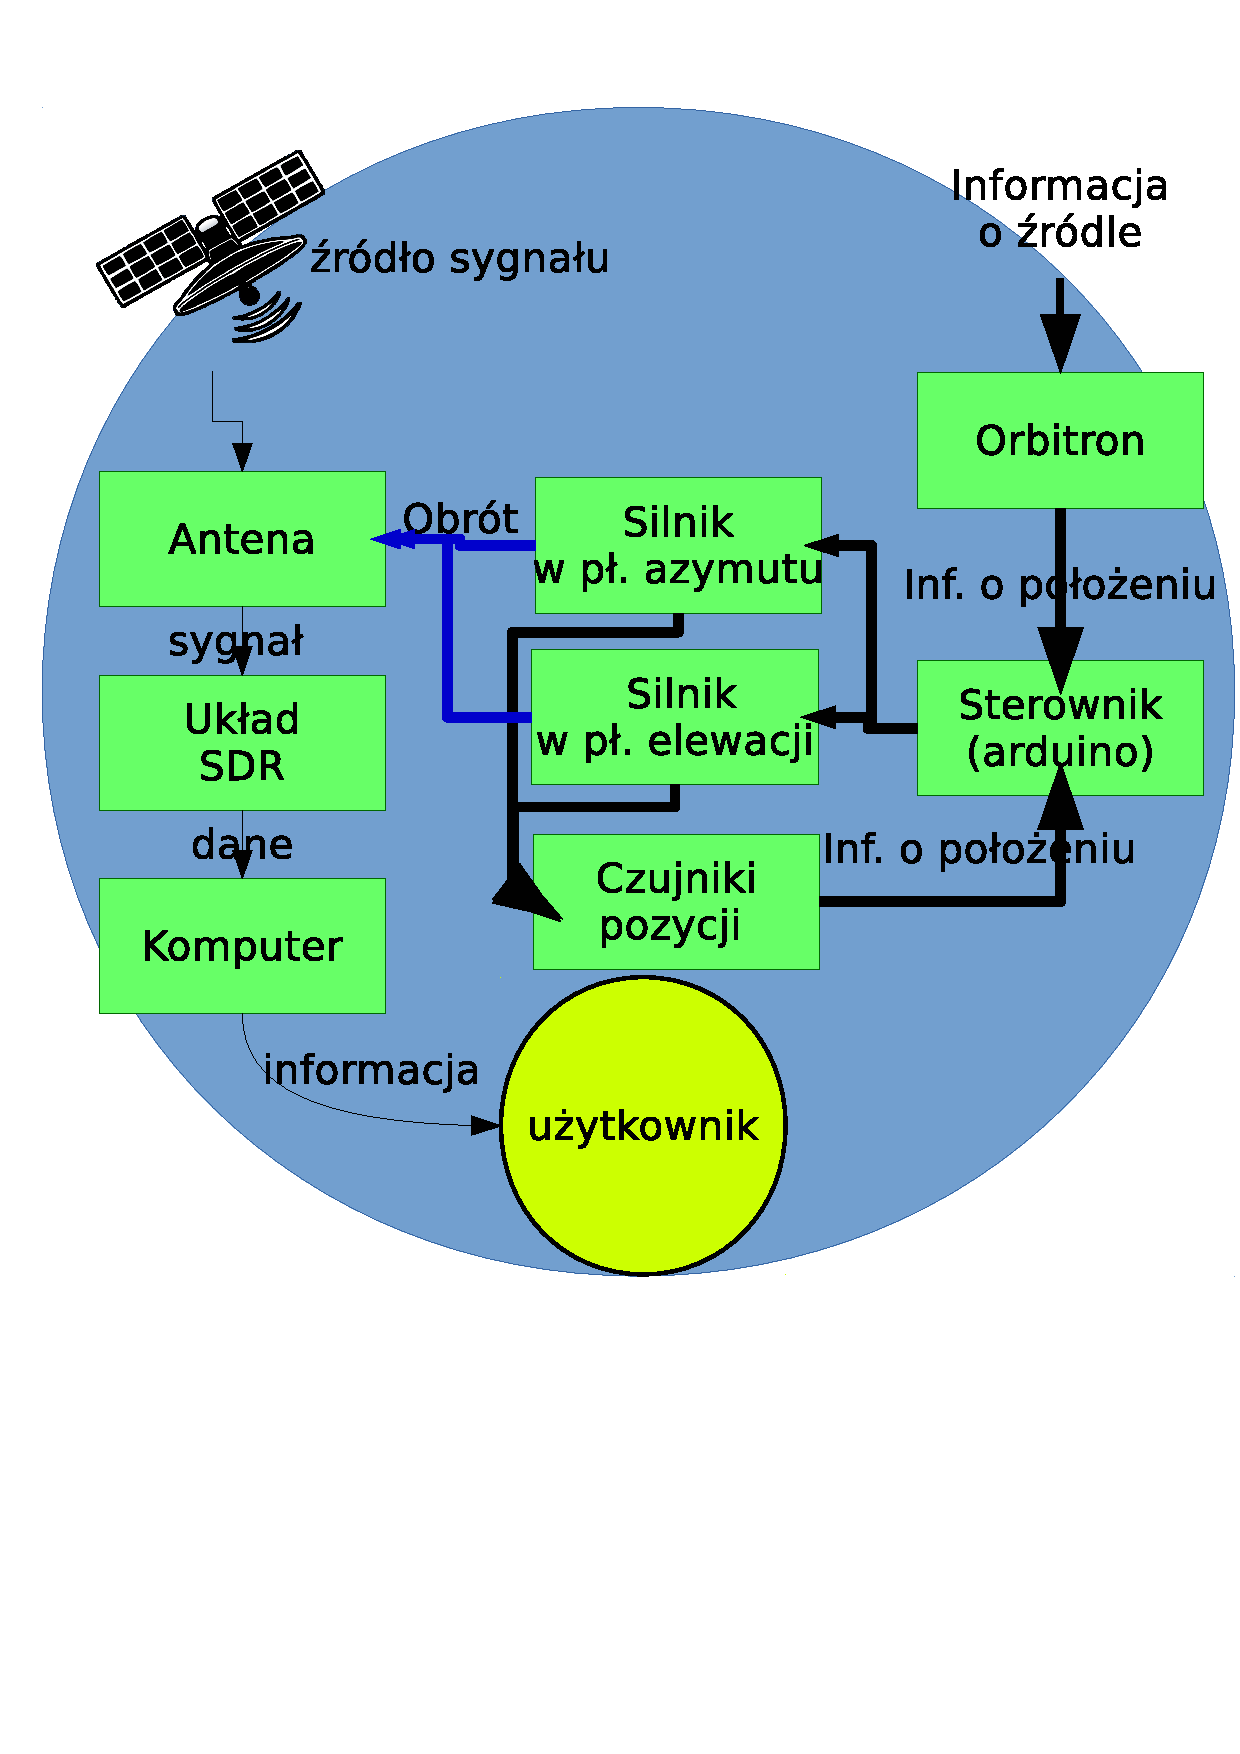
\includegraphics[width=0.8\textwidth]{schemat_skik2017}
    \caption{Schemat blokowy systemu stacji naziemnej}
\end{figure}

\section{Rotor do sterowania antenami w płaszczyźnie azymutu i elewacji}

Konstrukcja rotora składa się z dwóch stalowych skrzynek osłaniających silniki. W skrzynkach zostały wykonane otwory na poprowadzenie przewodów do zasilania i sterowania.

Aby uzyskać system z dużą precyzją i wytrzymały na warunki zewnętrzne pomimo małych gabarytów, potrzebne było duże przełożenie dla silników. Po doborze przekładni pełen obrót w płaszczyźnie azymutu zajmuje 124 sekundy, a w płaszczyźnie elewacji 64 sekundy. Wolny czas obrotu zwykle w rotorach antenowych nie przeszkadza, ponieważ zwykle nie namierza się szybko poruszających się źródeł sygnału. Podane prędkości są dla zasilania napięciem 12 V. Jest możliwe uzyskanie proporcjonalnie szybszych obrotów dostarczając większe napięcie zasilania (np. łącząc dwa akumulatory równolegle). Użyte silniki tolerują napięcie do 30V.

Zastosowane przekładnie wprost za silnikami mają mechanizm samoblokujący - ślimakowy, co uniemożliwia ich obrotu bez pracy silników.

Śledzenie pozycji rotora odbywa się przy pomocy zestawu czujników: 
\begin{itemize}
 \item enkoderów optycznych przed przekładnią (co znacznie poprawia ich rozdzielczość na pełen obrót, ale wprowadza trochę błędu ze względu na luzy w przekładniach)
 \item zamontowanego do osi z na anteny układu czujników \emph{pololu} zawierającego kompas magnetyczny, żyroskopy i akcelerometry w trzech osiach, który służy do kalibracji układu.
\end{itemize}

Kalibracja układu polega na ustaleniu na podstawie danych z kompasu aktualnej orientacji rotora względem kierunków geograficznych. Wcześniejsze relatywne położenie rotora jest odczytywane z pamięci stałej EEPROM. Podczas kalibracji wykonuje się też pełen obrót w płaszczyźnie azymutu i wykrywa się przy pomocy akcelerometru czy rotor nie stoi pochylony. W przypadku wykrycia pochyłu do zadawanych położeń obliczana jest dodatkowa korekta.

\begin{figure}[!htbp]
 \includegraphics[width=0.8\textwidth]{rotor}
 \centering
 \caption{Konstrukcja rotora zamontowana na statywie}
\end{figure}

Cała stacja waży około 12 kilogramów. Rotor ma miejsce na przykręcane rury do mocowania anten. Przewidujemy nie więcej niż 2 anteny jednocześnie o łącznej wadze do 8 kilogramów.

Niestety tak jak w większości rotorów (poza zaawansowanymi rozwiązaniami), ze względu na kabel można obracać rotorem w wybranym kierunku tylko w ograniczonym zakresie. Maksymalny kąt obrotu zależy od poprowadzenia przewodu zarówno do anteny jak i zasilających w rotorze. Do zasilania daliśmy zapas kabla na około 2 pełne obroty. Pilnowanie aby nie przekroczyć maksymalnego obrotu odbywa się programowo zapamiętując i wczytując względny obrót w pamięci trwałej. 

Rotor bardzo trudno obrócić bez włączonego zasilania ze względu na duże przełożenie w przekładniach. Jest to zamierzone, aby przy trudniejszych warunkach atmoseferycznych (przede wszystkim wietrze) rotor się nie obracał bez kontroli.

Dolna część rotora zawiera silnik obracający część górną w płaszczyźnie azymutu przy pomocy dwóch przekładni - ślimakowej i planetarnej. W tym przypadku tarcza enkodera została zamontowana pomiędzy przekładniami ze względu na brak wyprowadzenia ośki silnika. Dolna skrzynka jest dość obszerna, żeby móc w środku schować układy elektroniczne (sterownik arduino, mostki H, przetwornica napięcia). Ta część zawiera też otwory na przewody do komputera na kabel USB i przewody do zasilania. Dolna część rotora bez układów elektornicznych została przedstawiona na rysunku \ref{rotdol}.

Górna część rotora znajdująca się na rysunku \ref{rotgora} zawiera silnik obracający oś do mocowania anten w płaszczyźnie elewacji. Do skrzynki dochodzą przewody z dolnej części - przewody: zasilający 12V, zasilający 5V, masy, 2 sterujące silnikiem i przewód z danymi enkodera. Wszystko jest umieszczone w jednym kablu 6-żyłowym skręconym, aby był elastyczny i rozciągliwy. 

W przenośnym rozwiązaniu układ SDR znajduje się w dodatkowym pokrowcu (walizce) umieszczonym pod rotorem, gdzie dochodzi do niego przewód radiowy wprost z anteny.

W rozwiązaniu zrezygnowano z użycia silników krokowych w zamian za proste silniki szczotkowe DC wraz z dodaniem enkoderów, ze względu na łatwość uzyskania dobrej precyzji tanim kosztem. W ramach projektu opracowano też sterowniki do silników w postaci mostków H. Schemat układu przedstawiono na rysunku \ref{mostekh}.

\begin{figure}[!htbp]
 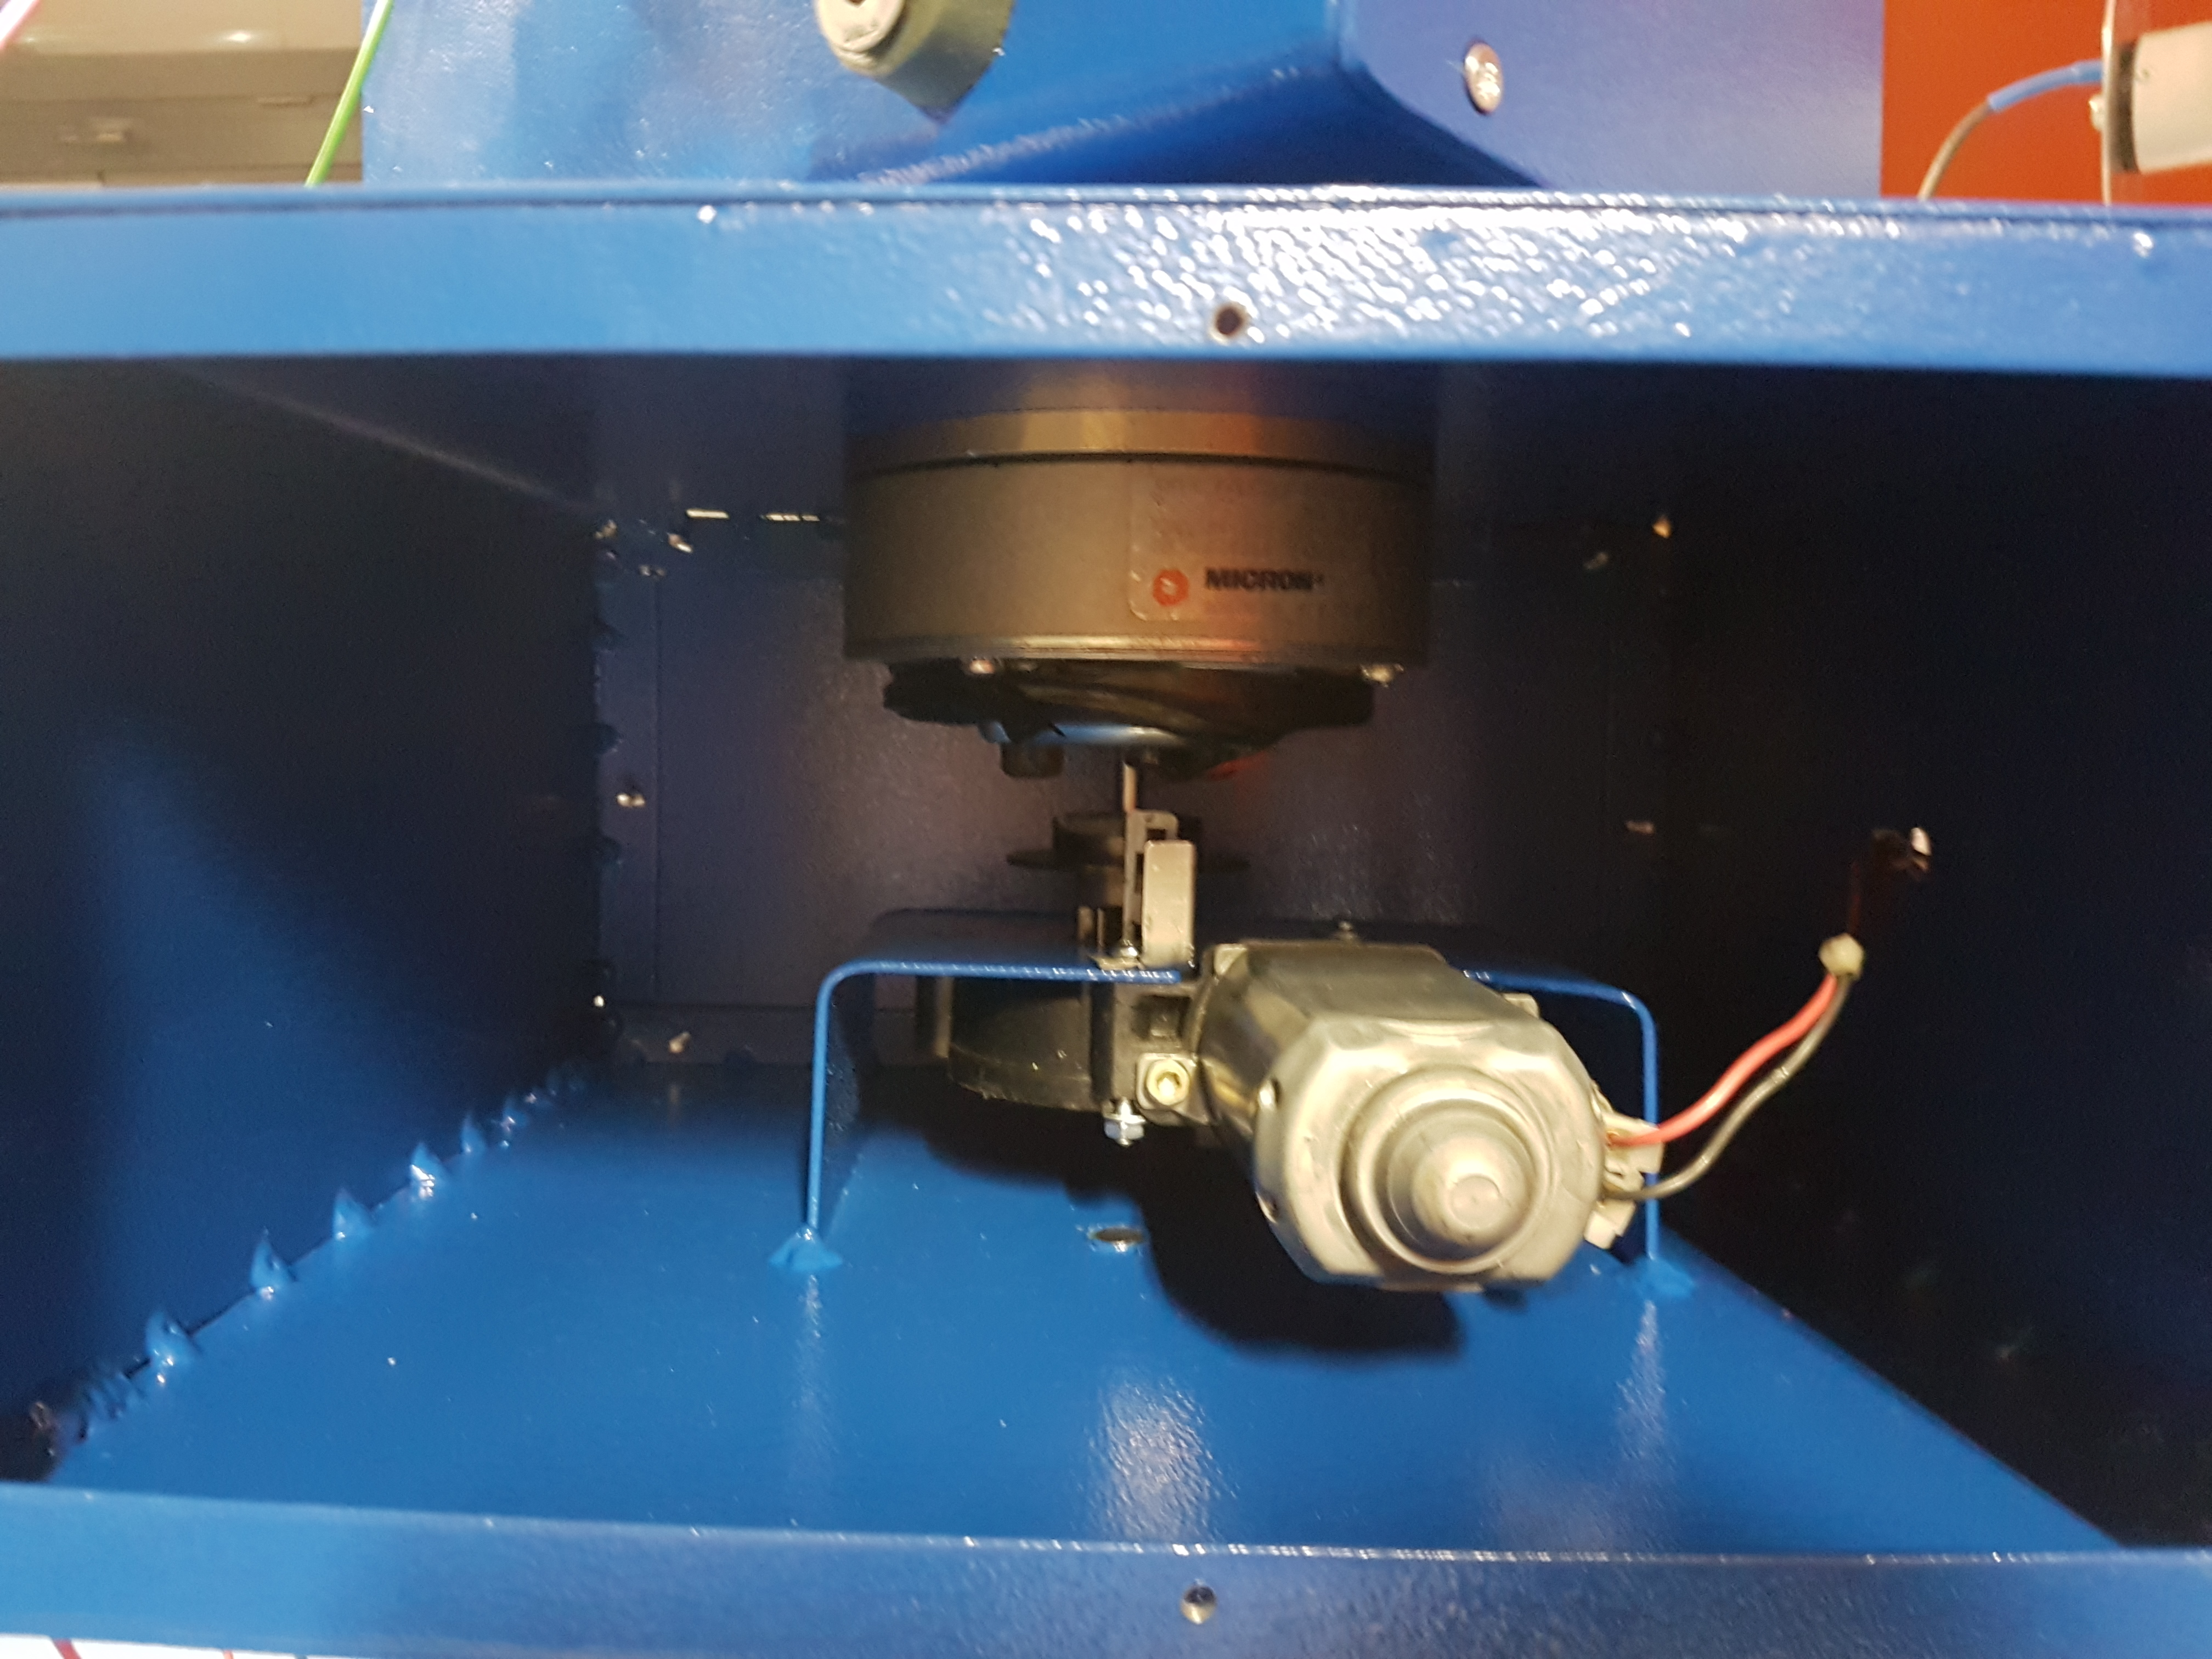
\includegraphics[width=\textwidth]{rotor_dol}
 \centering
 \caption{Wnętrze dolnej części rotora}
 \label{rotdol}
\end{figure}

\begin{figure}[!htbp]
 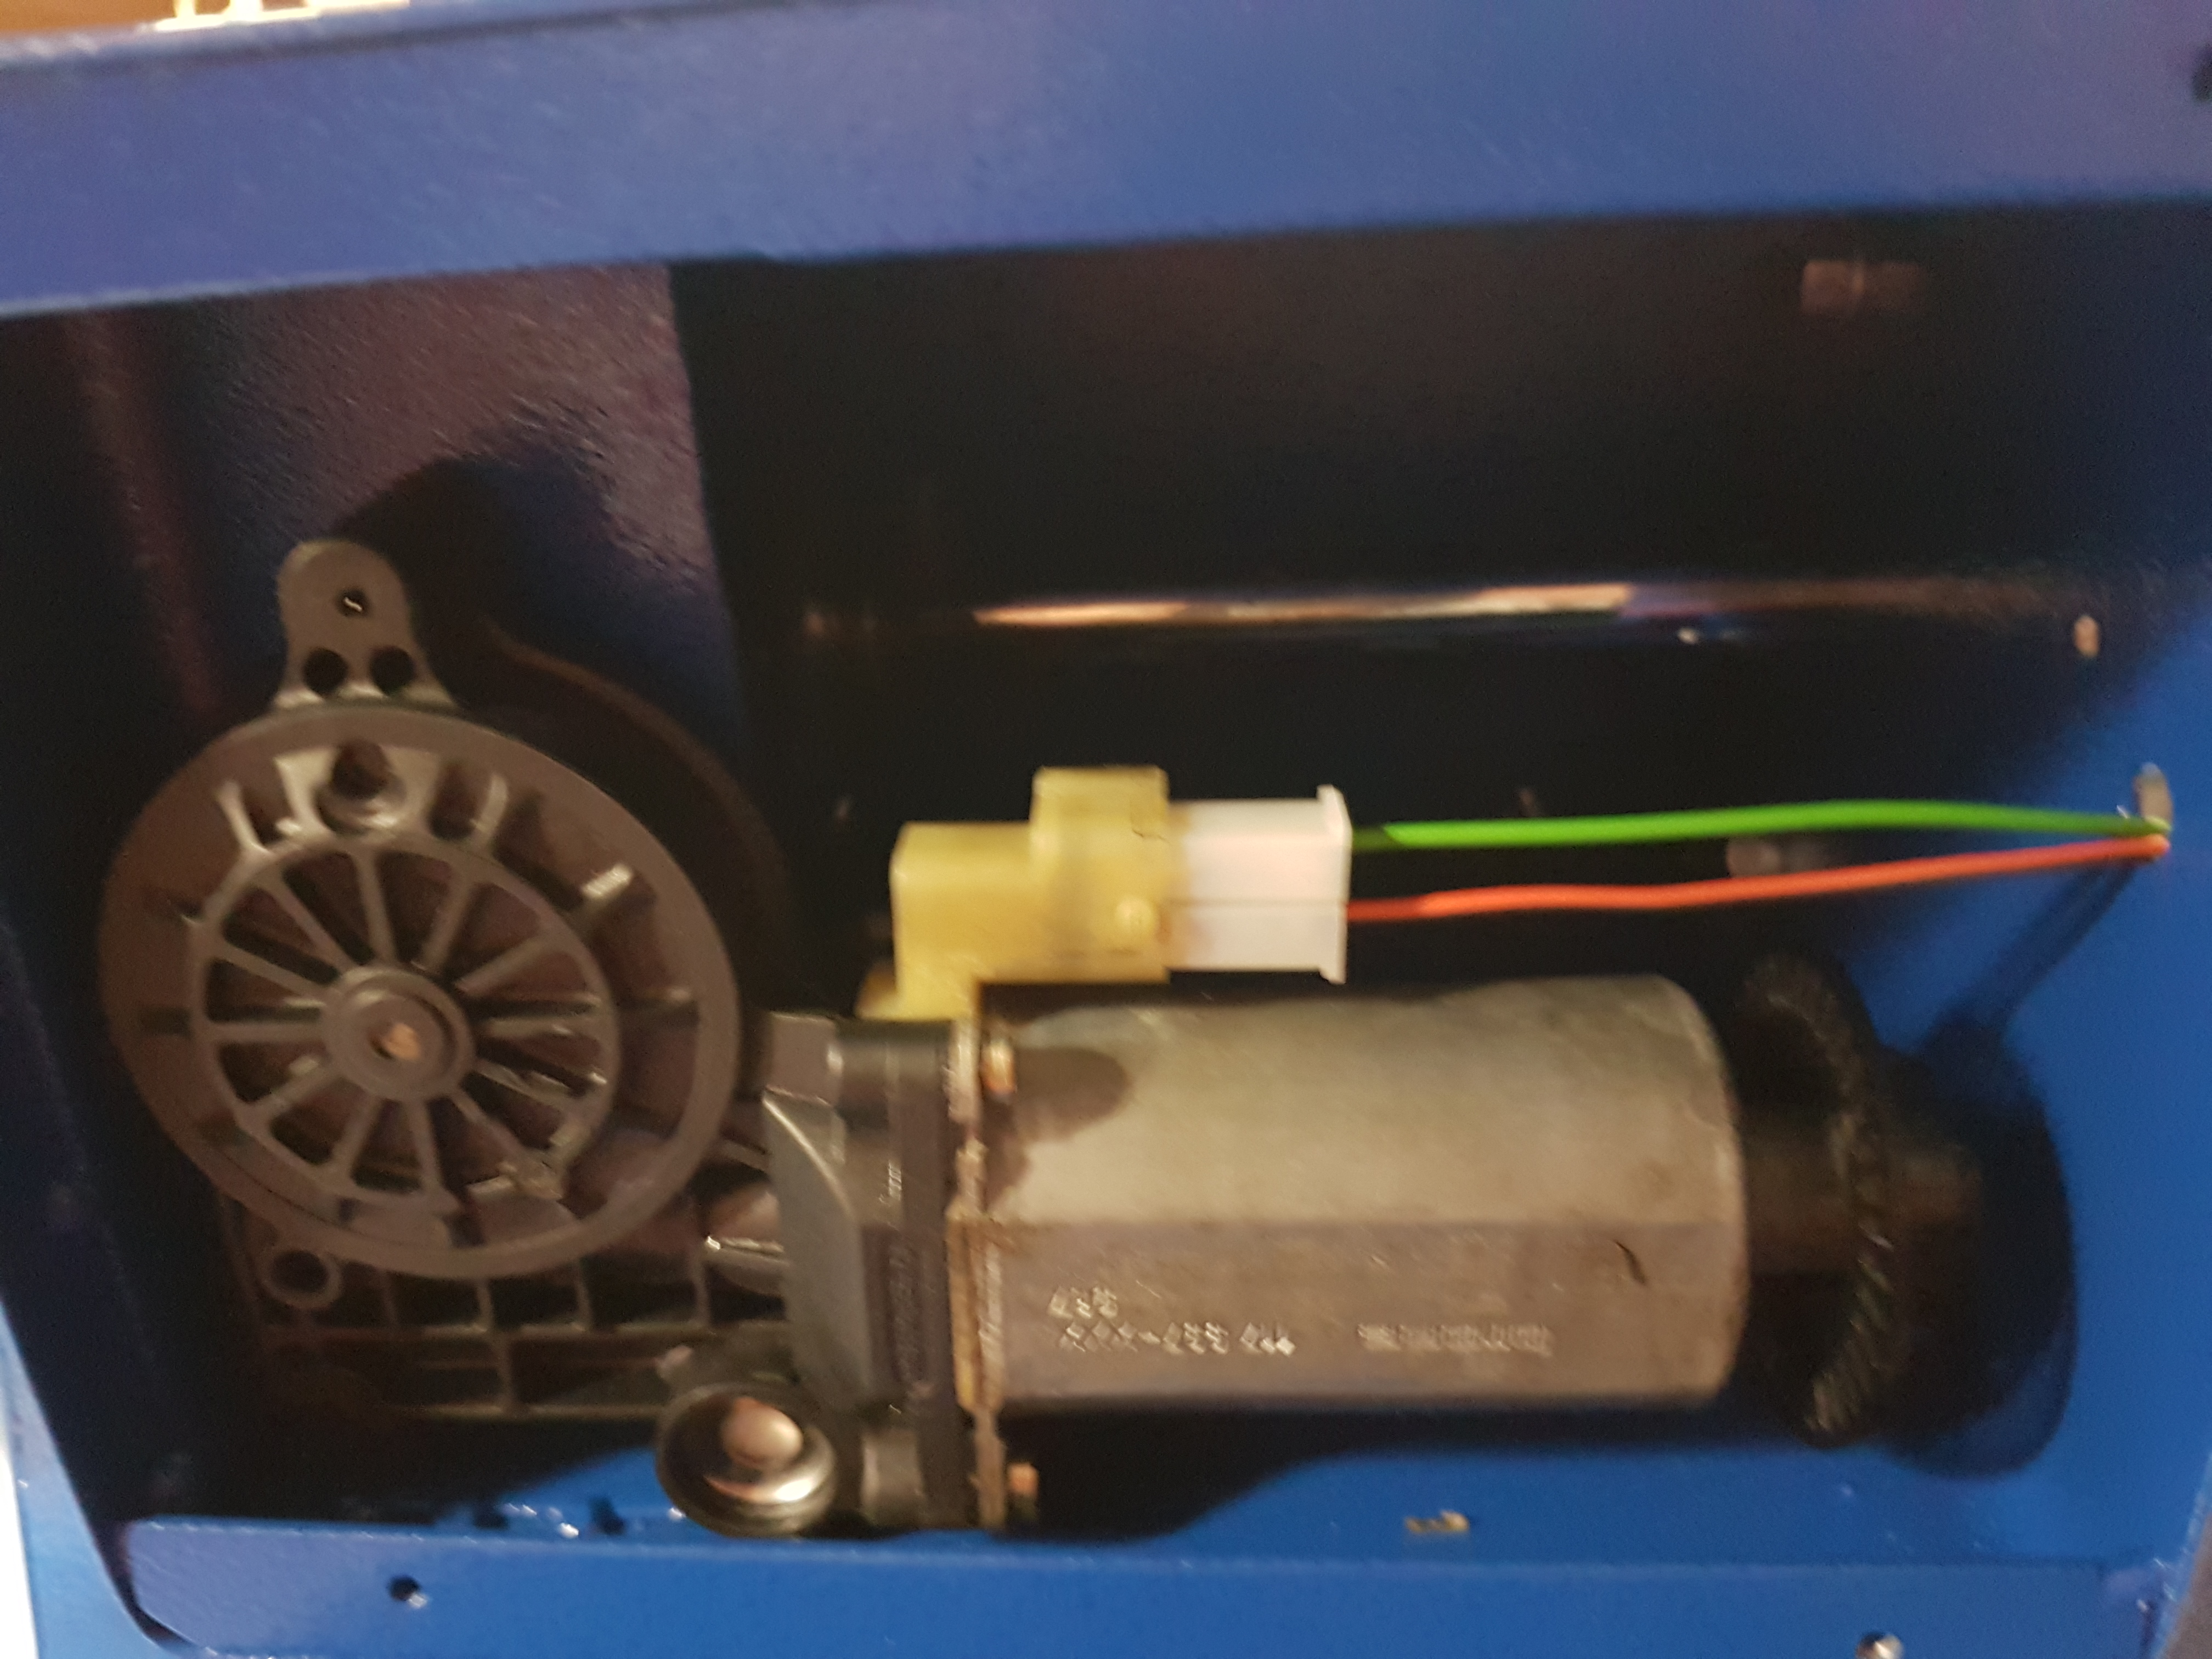
\includegraphics[width=\textwidth]{rotor_gora}
 \centering
 \caption{Wnętrze górnej części rotora}
 \label{rotgora}
\end{figure}

\begin{figure}[!htbp]
 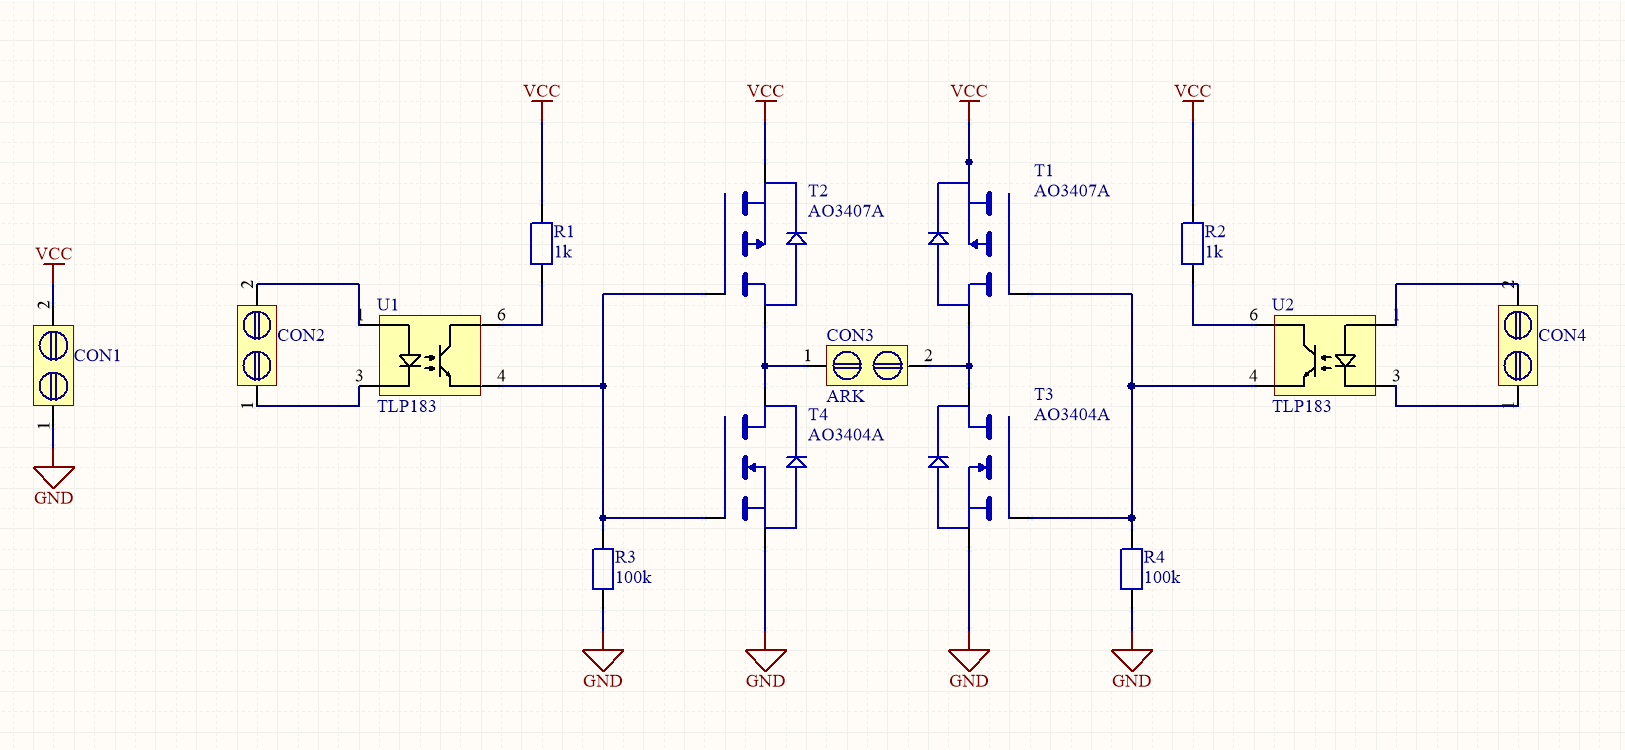
\includegraphics[width=\textwidth]{mostekh}
 \centering
 \caption{Mostek H - układ do sterowania silnikiem DC}
 \label{mostekh}
\end{figure}

\section{Sterowanie}

Do sterowania rotorem wykorzystano możliwości programu Orbitron, który pozwala śledzić ruch satelit poruszających się na orbicie okołoziemskiej. Użytkownik jest w stanie otrzymać informacje o położeniu danego satelity na orbicie oraz wysyłać komunikaty z informacją o kącie azymutu i elewacji anteny jaki należy ustawić, żeby namierzyć wybranego satelitę. Na Rys. \ref{fig:rotor} poniżej zamieszczono widok ekranu głównego aplikacji. 

\begin{figure}[h]
	\centering
		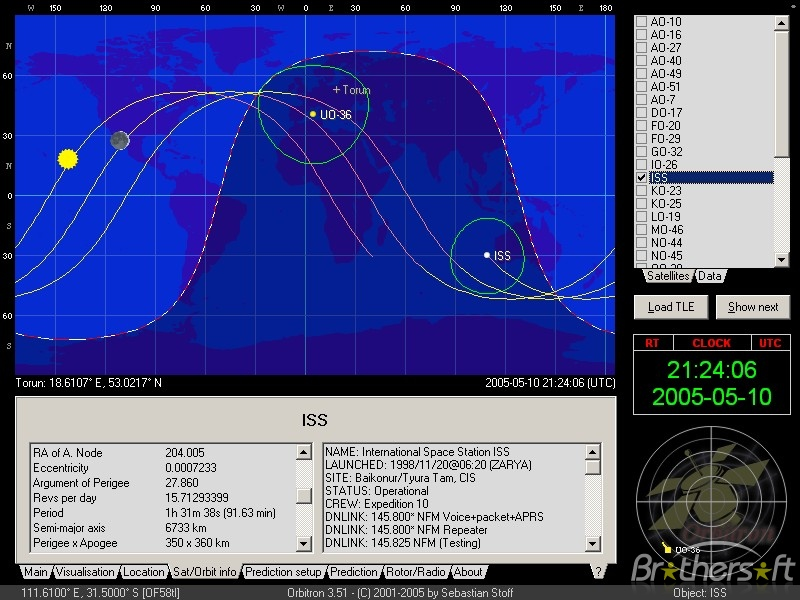
\includegraphics[width=0.7 \textwidth]{orbitron}
	\caption{Widok ekranu głównego programu Orbitron}	
	\label{fig:rotor}
\end{figure}

Aby nawiązać komunikację z układem sterującym rotorami zainstalowano aplikację, będącą dodatkiem do programu Orbitron - \textit{DDE Orbitron To Serial} \cite{dde}. Program na bieżąco może pobierać informacje o położeniu satelit i wysyłajać komunikaty poprzez port szeregowy do układu sterującego rotorem.


\begin{figure}[h]
	\centering
		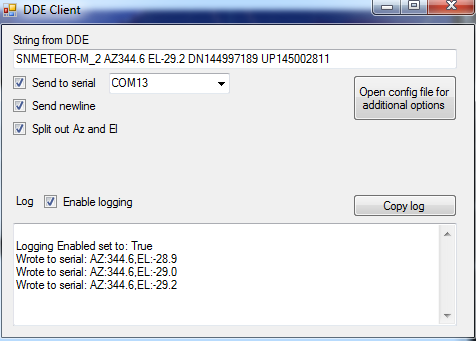
\includegraphics[width=0.7 \textwidth]{DDEOrbitronToSerialScreenShot}
	\caption{Widok okienka aplikacji DDE Orbitron To Serial}	
	\label{fig:rotor}
\end{figure}

Komunikaty z informacją o kącie elewacji i azymutu anteny są wysyłane bezpośrednio do sterownika (płytki Arduino Uno). Program mikrokontrolera umożliwia sterowanie dwoma silnikami rotora oraz jako sprzężenie zwrotne odbiera dane z enkoderów umieszczonych na osiach silników. Mikrokontroler zlicza impulsy odebrane z czujników co daje pełną informację o rzeczywistym ustawieniu anteny i umożliwia ewentualną korektę. Silniki rotora są silnikami prądu stałego z przekładnią i pozwalają na obrót ze stałą prędkością, więc aby obrócić oś o określony kąt zbadano jaka ilość impulsów enkodera odpowiada pełnemu obrotowi. 

\section{Część radiowa}

% Do wykonania przetwarzania w części radiowej wykorzystaliśmy radio

Radio które posiadaliśmy w laboratorium USRP-2932 niestety nie nadaje się do odbioru sygnału APRS ze względu na dolną granicę pasma 400 MHz. Zamiast tego wykorzystaliśmy je do odbioru transmisji o modulacji LoRa wykorzystując jako nadajnik układ z poprzedniego projektu: Orange Pi połączony z układem nadawczym. Do testów transmisji APRS wykorzystaliśmy inne radio programowalne.

Dodatkowo jeden z członków podjął się wykonania części odbiornika (samej demodulacji) na układzie FPGA z przetwornikiem analogowo-cyfrowym. Niestety nie możemy wykorzystać tego rozwiązania, ponieważ brakuje synchronizacji i części analogowej (filtry, mieszacz).

\begin{figure}[!htbp]
 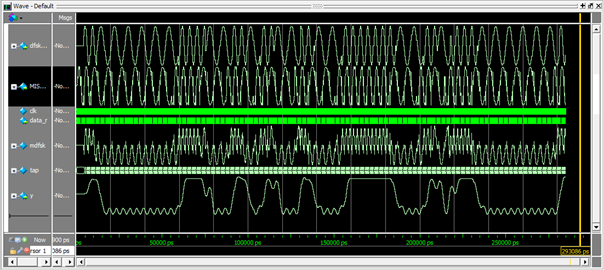
\includegraphics[width=0.8\textwidth]{symulacja}
 \centering
 \caption{Wynik symulacji demodulacji APRS na FPGA}
\end{figure}

Okazało się, że gotowe projekty oprogramowania demodulatora zarówno APRS jak i LoRa są dostępne w internecie z otwartym oprogramowaniem w GNU radio, więc wystarczyło je przetestować w naszych układach.

\section{Podsumowanie i testy stacji}

Testy stacji stanowiły testy części radiowej i konstrukcyjnej. W ramach grantu kupiono balon na misję balonową, aby wraz z układem z poprzedniego grantu przetestować łącze radiowe w praktycznych warunkach.

\subsection{Test współpracy z oprogramowaniem Orbitron}

W celów testu wyznaczyliśmy w programie symulowany przelot stacji ISS w okolicach Warszawy i włączyliśmy nasz sterownik do wodzenia anteną za stacją ISS będącą najszybciej poruszającym się obiektem na bliskiej orbicie.

Oprogramowanie zadziałało poprawnie i stacja była sterowana za pośrednictwem komputera. W tym teście okazało się, że stacja ISS przy bliskim przelocie jest znacząco zbyt szybko poruszającym się obiektem dla naszego rotora. Rotor nadążął za zmianami w płaszczyźnie elewacji, ale zmiany azymutalne były zbyt duże. Jak wcześniej wspomniano, można przyspieszyć obroty zwiększając napięcie, ale ogólnie nie przewidywaliśmy śledzenia tak szybkich obiektów. Na zakończenie kilkunastosekundowego testu zrobiliśmy pomiar zewnętrznym kompasem. Jest to przedstawione na rysunku \ref{kompas}.

Test orientacji w płaszczyźnie azymutu wykazał błąd na poziomie $\pm 3^o$, ze względu na niską dokładność użytego kompasu w module. Z drugiej strony potencjalna rozdzielczość rotora w jednostce na impuls enkodera wynosi $0.02^o$ w płaszczyźnie elewacji i $0.2^o$ w płaszczyźnie azymutu dzięki wolnym obrotom. W związku z tym dodaliśmy opcję ręcznego wprowadzenia kalibracji orientacji z komputera jeśli zajdzie potrzeba uzyskania większej dokładności.

Wykonaliśmy test obrotu dookoła, aby sprawdzić czy sterownik steruje poprawnie i nie zerwie kabla sterownika. Rotor poprawnie zaprogramowany nie zerwał kabla i zaczął obracać się w przeciwnym kierunku (o ujemny kąt) aby wykonać pełen obrót.
% 
% \begin{figure}[h]
% 	\centering
% 		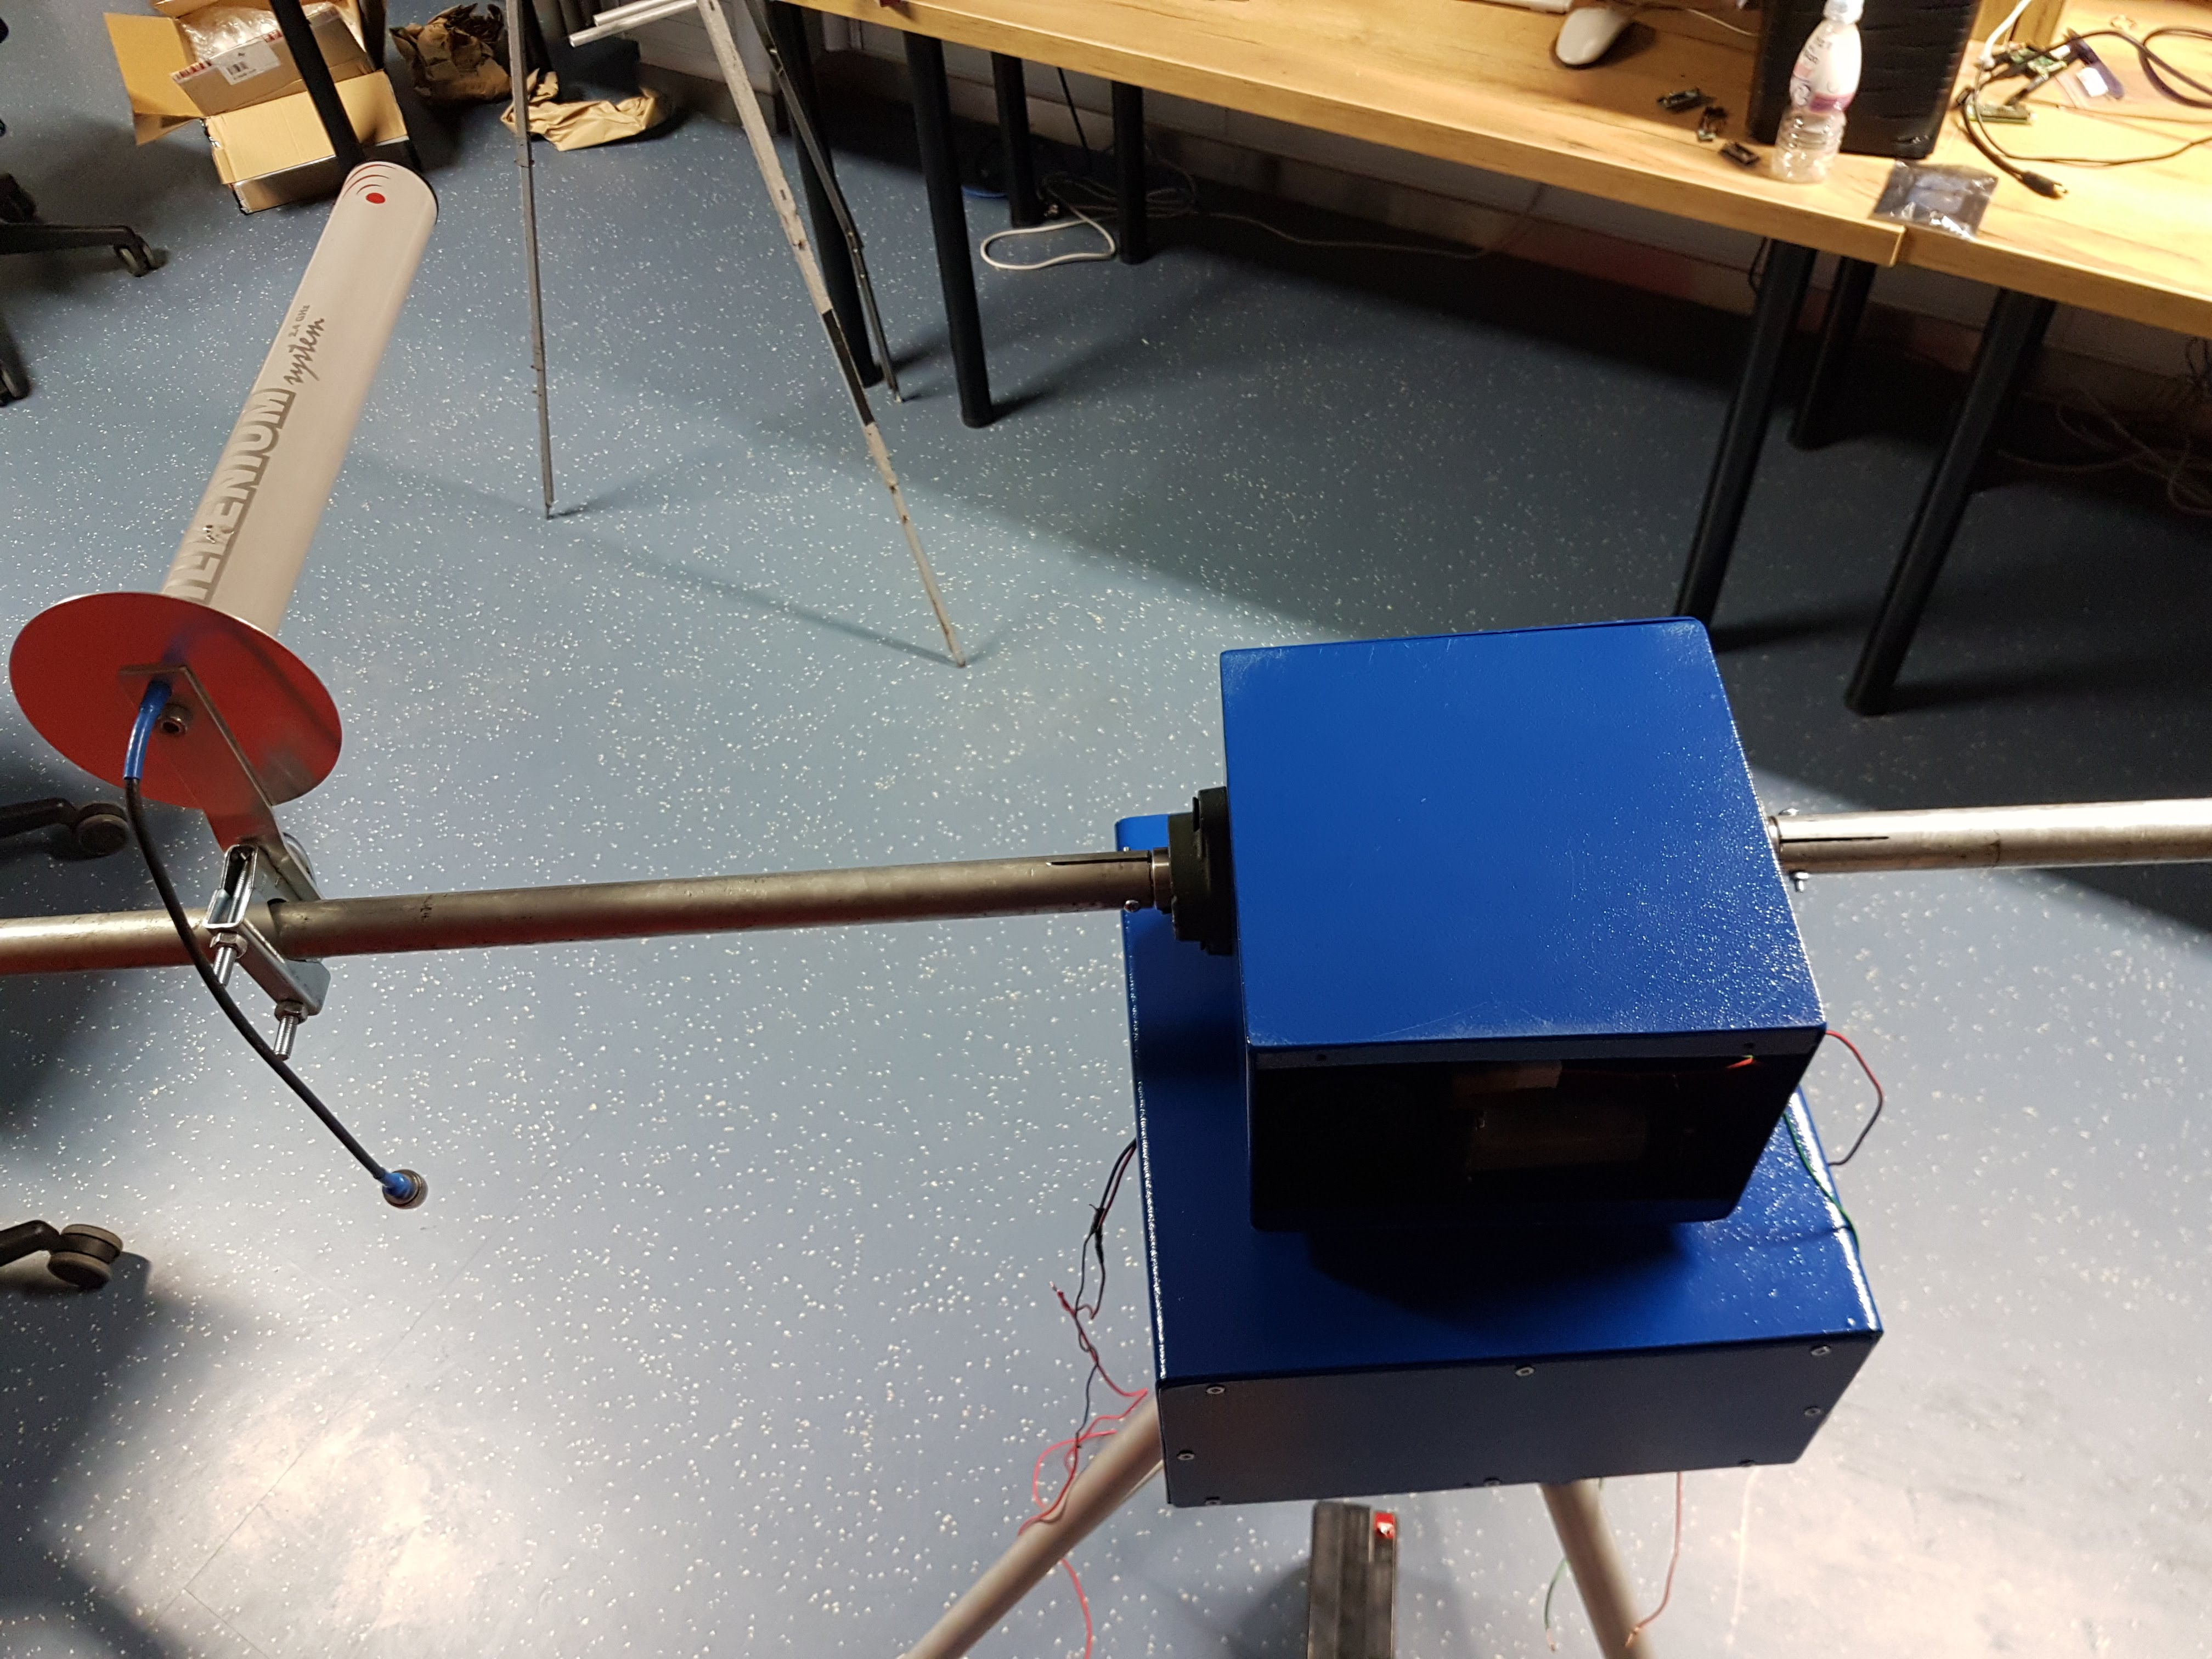
\includegraphics[width=0.7 \textwidth]{testy/antenaS}
% 	\caption{Antena wskazuje kierunek południowy}	
% 	\label{fig:antenaS}
% \end{figure}
% 
% \begin{figure}[h]
% 	\centering
% 		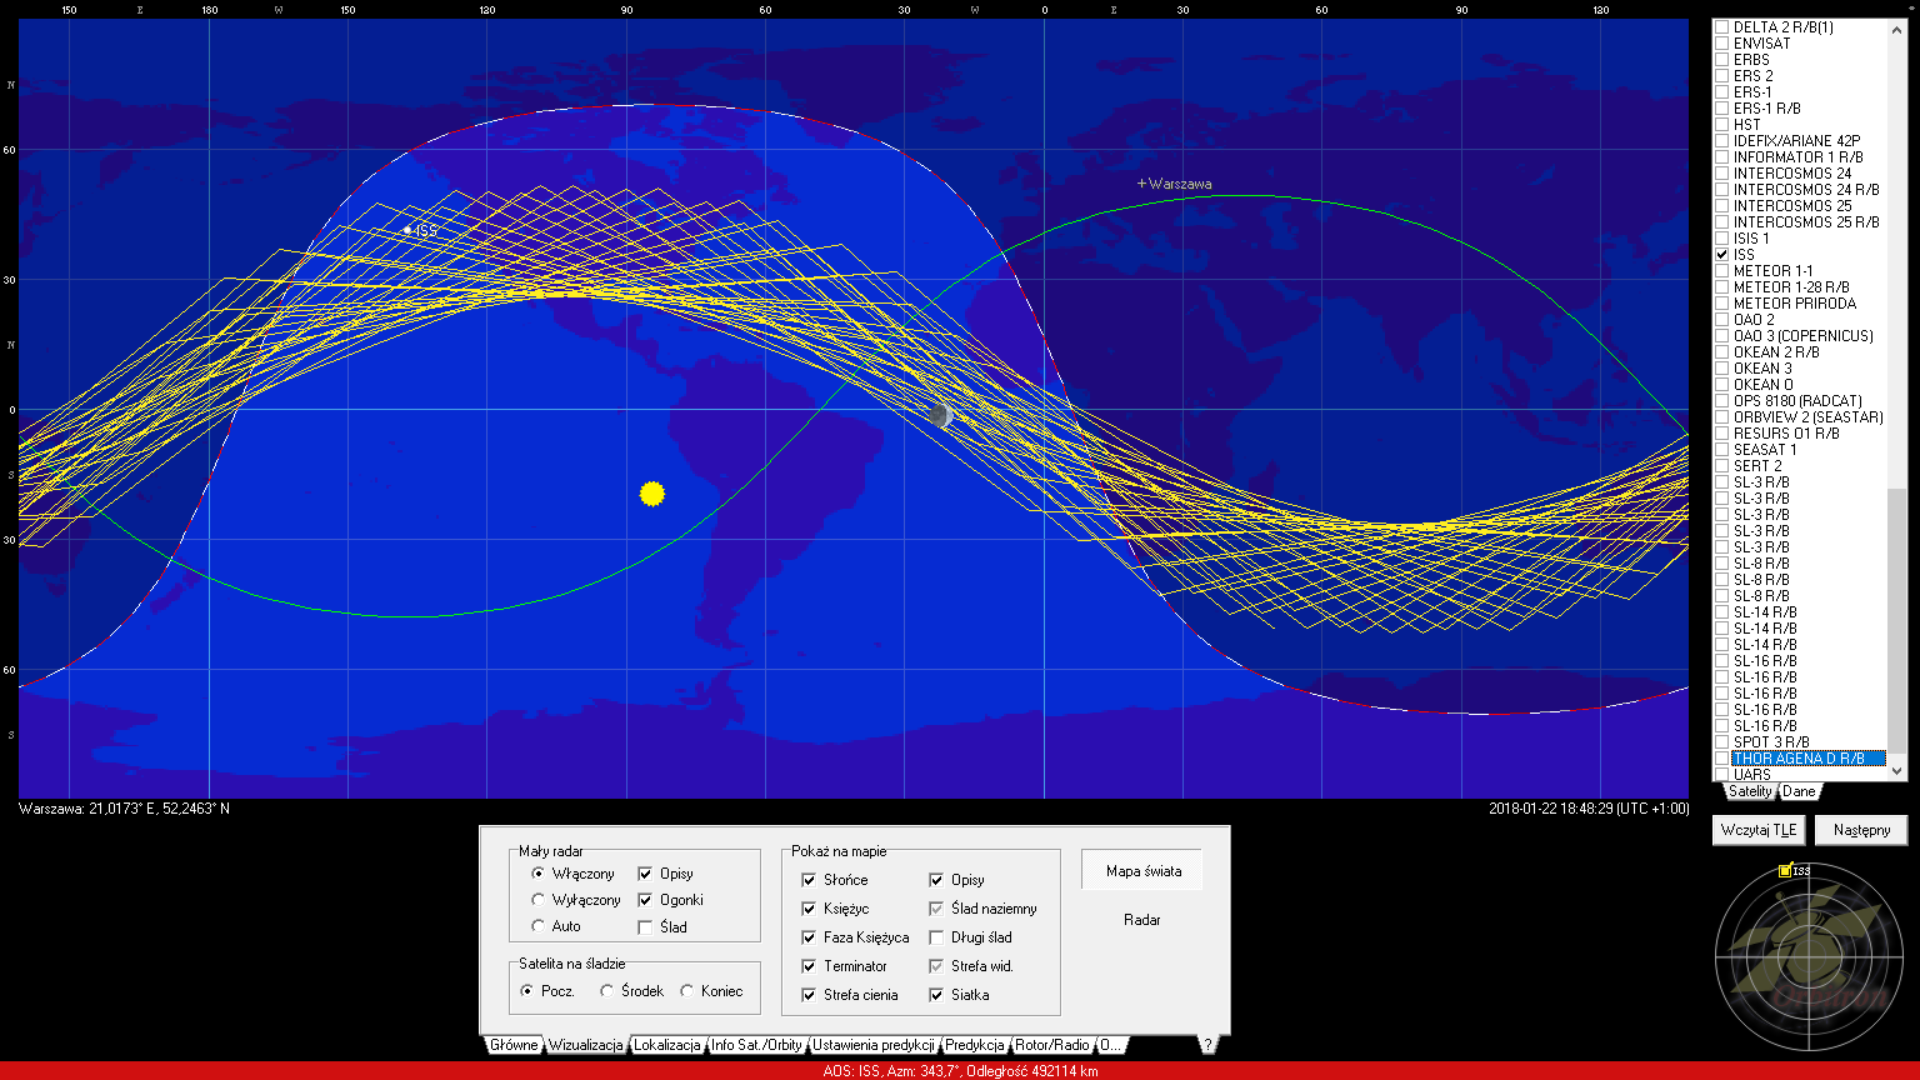
\includegraphics[width=0.7 \textwidth]{testy/pojawia}
% 	\caption{Satelita ISS pojawia się nad horyzontem}	
% 	\label{fig:pojawia}
% \end{figure}
% 
% \begin{figure}[h]
% 	\centering
% 		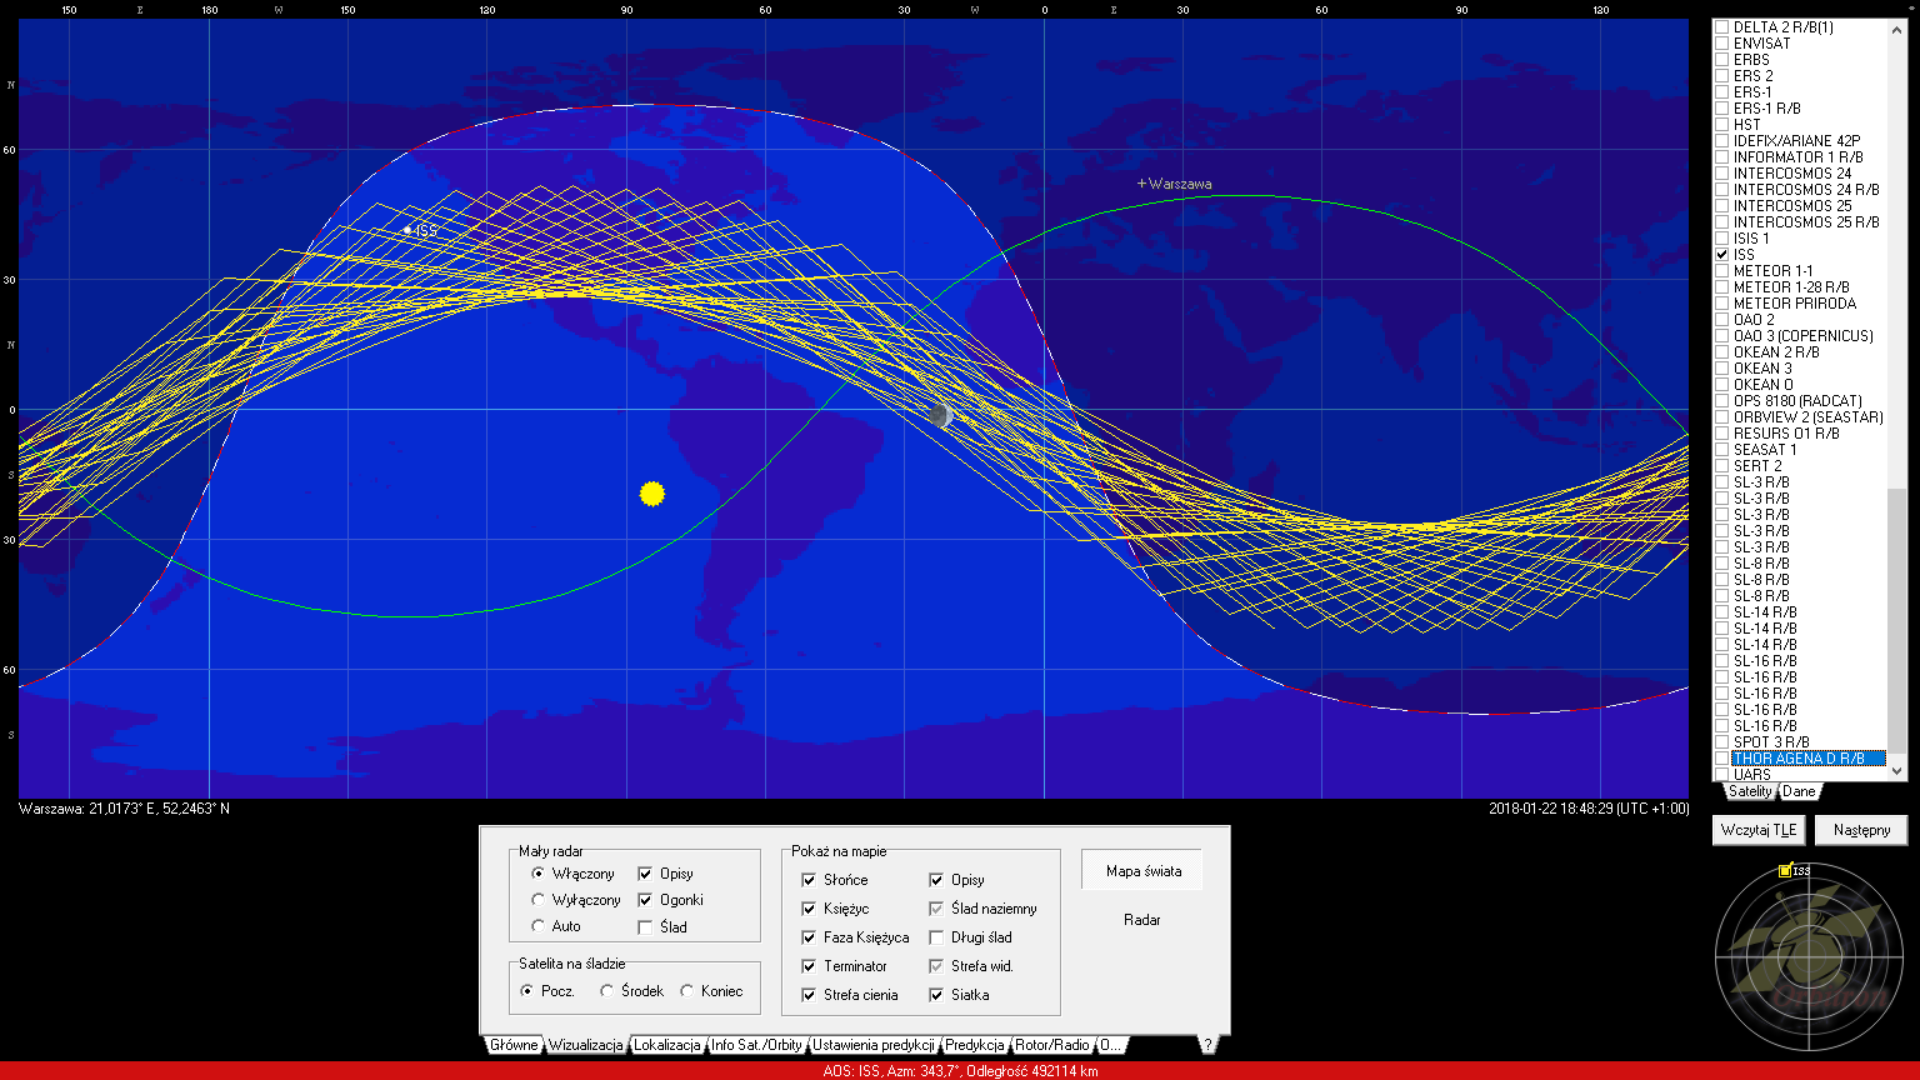
\includegraphics[width=0.7 \textwidth]{testy/pojawia}
% 	\caption{Satelita ISS pojawia się nad horyzontem}	
% 	\label{fig:pojawia}
% \end{figure}
% 
% 
% \begin{figure}[h]
% 	\centering
% 		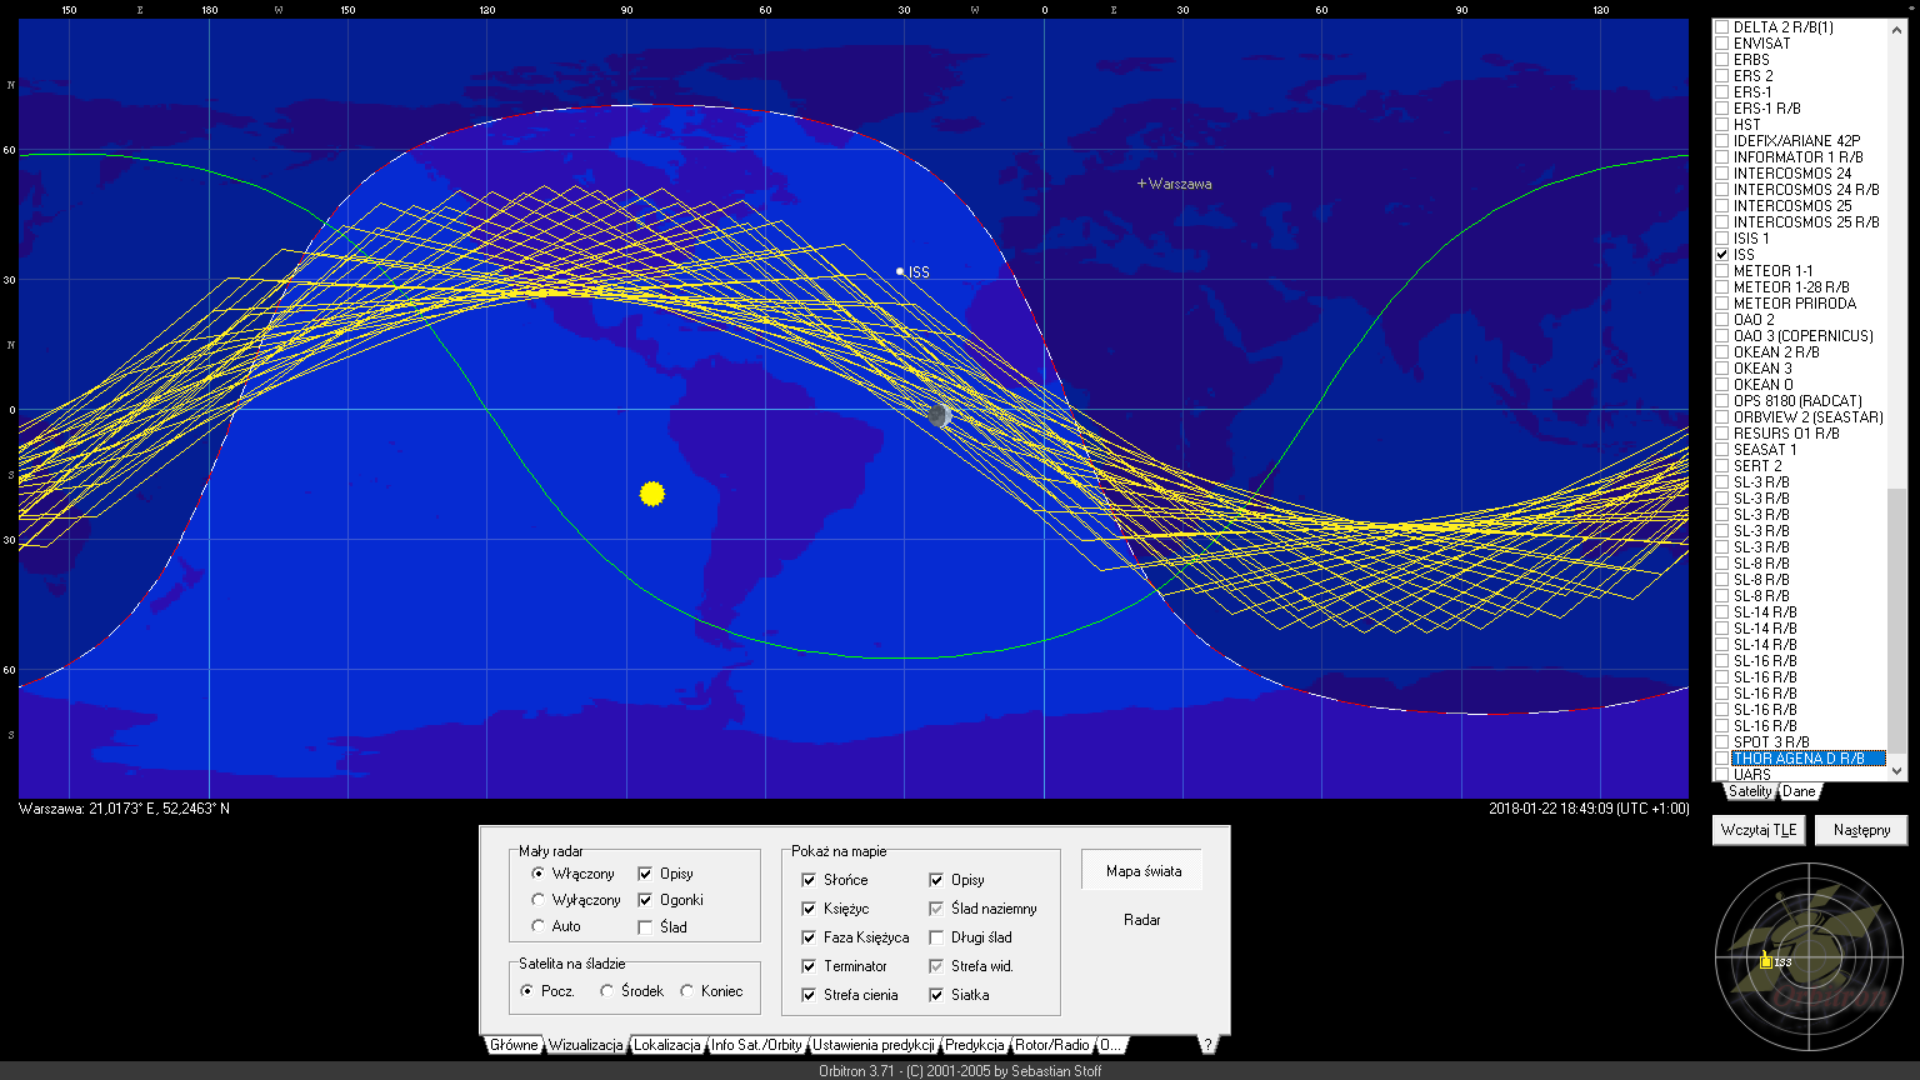
\includegraphics[width=0.7 \textwidth]{testy/zenit}
% 	\caption{Satelita ISS w zenicie}	
% 	\label{fig:zenit}
% \end{figure}
% 
% 
% \begin{figure}[h]
% 	\centering
% 		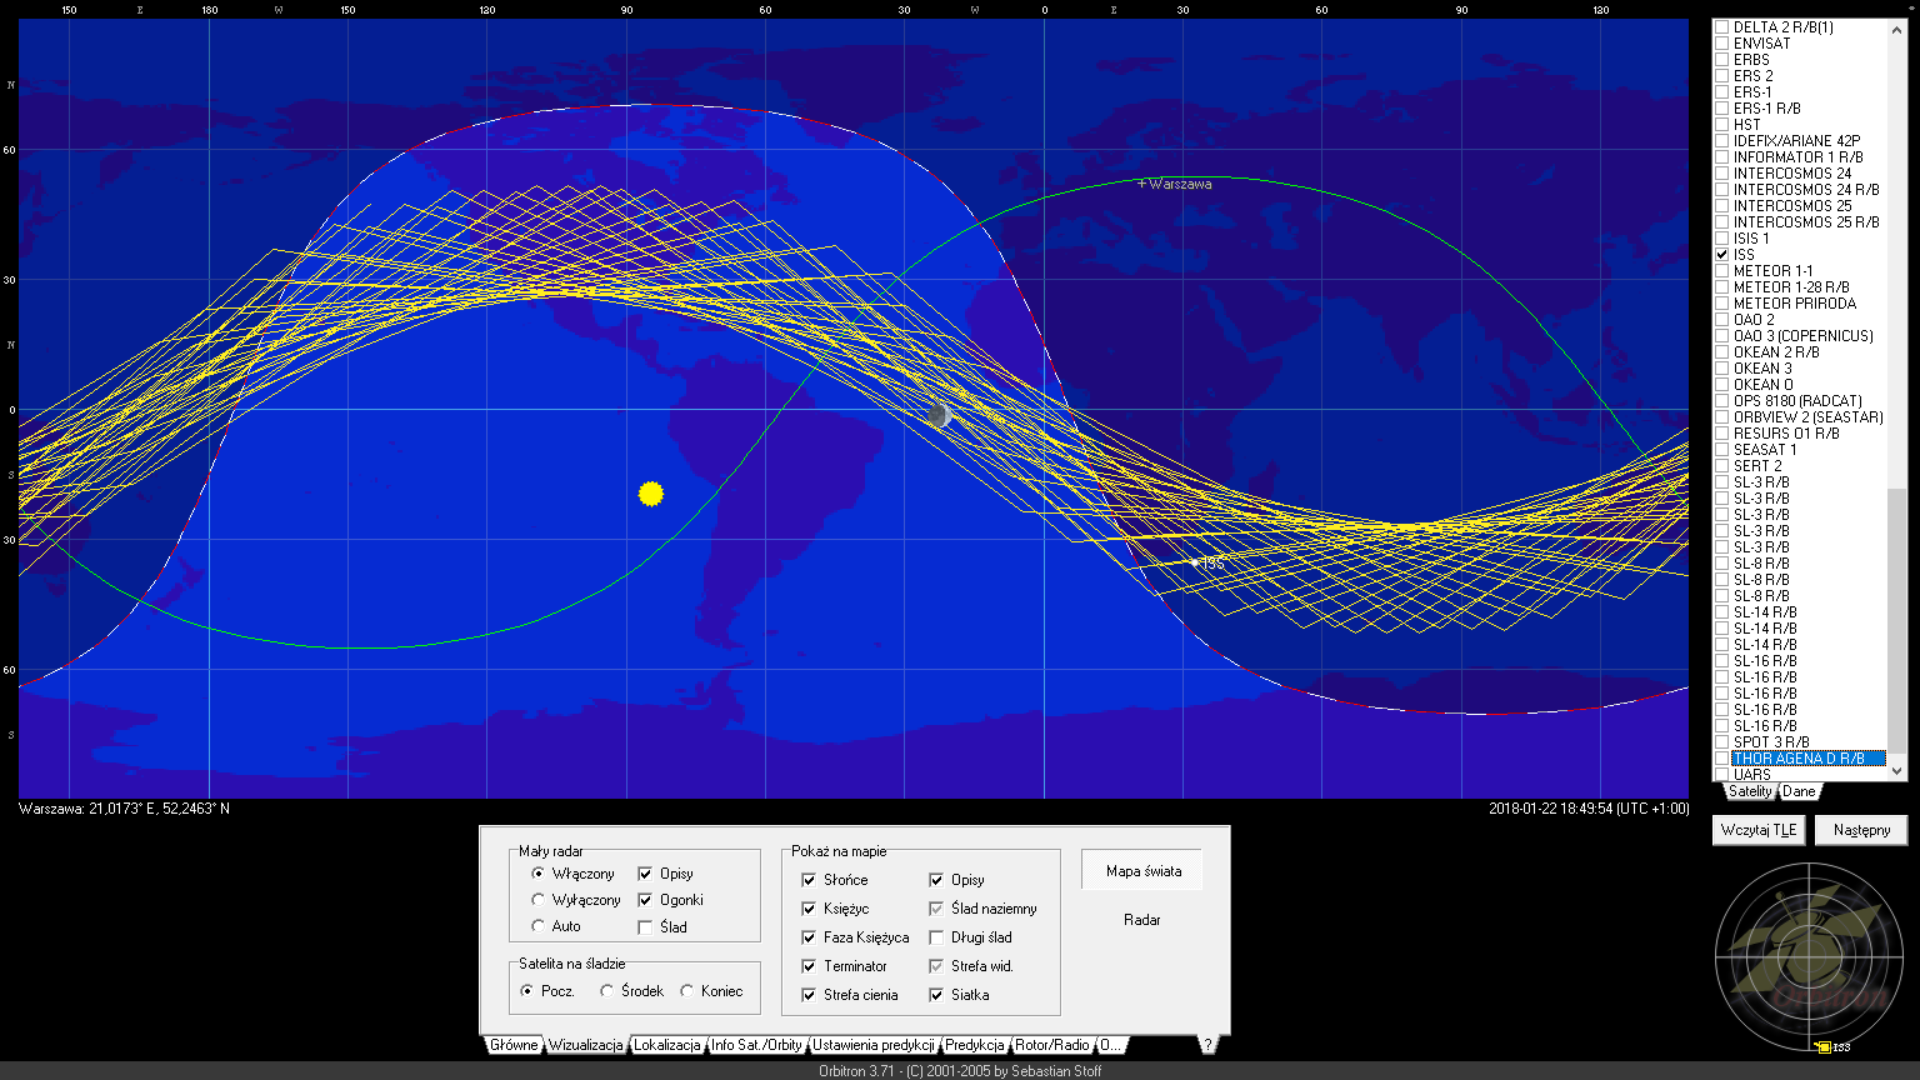
\includegraphics[width=0.7 \textwidth]{testy/znika}
% 	\caption{Satelita ISS znika za horyzontem}	
% 	\label{fig:zanika}
% \end{figure}


\begin{figure}[!htbp]
 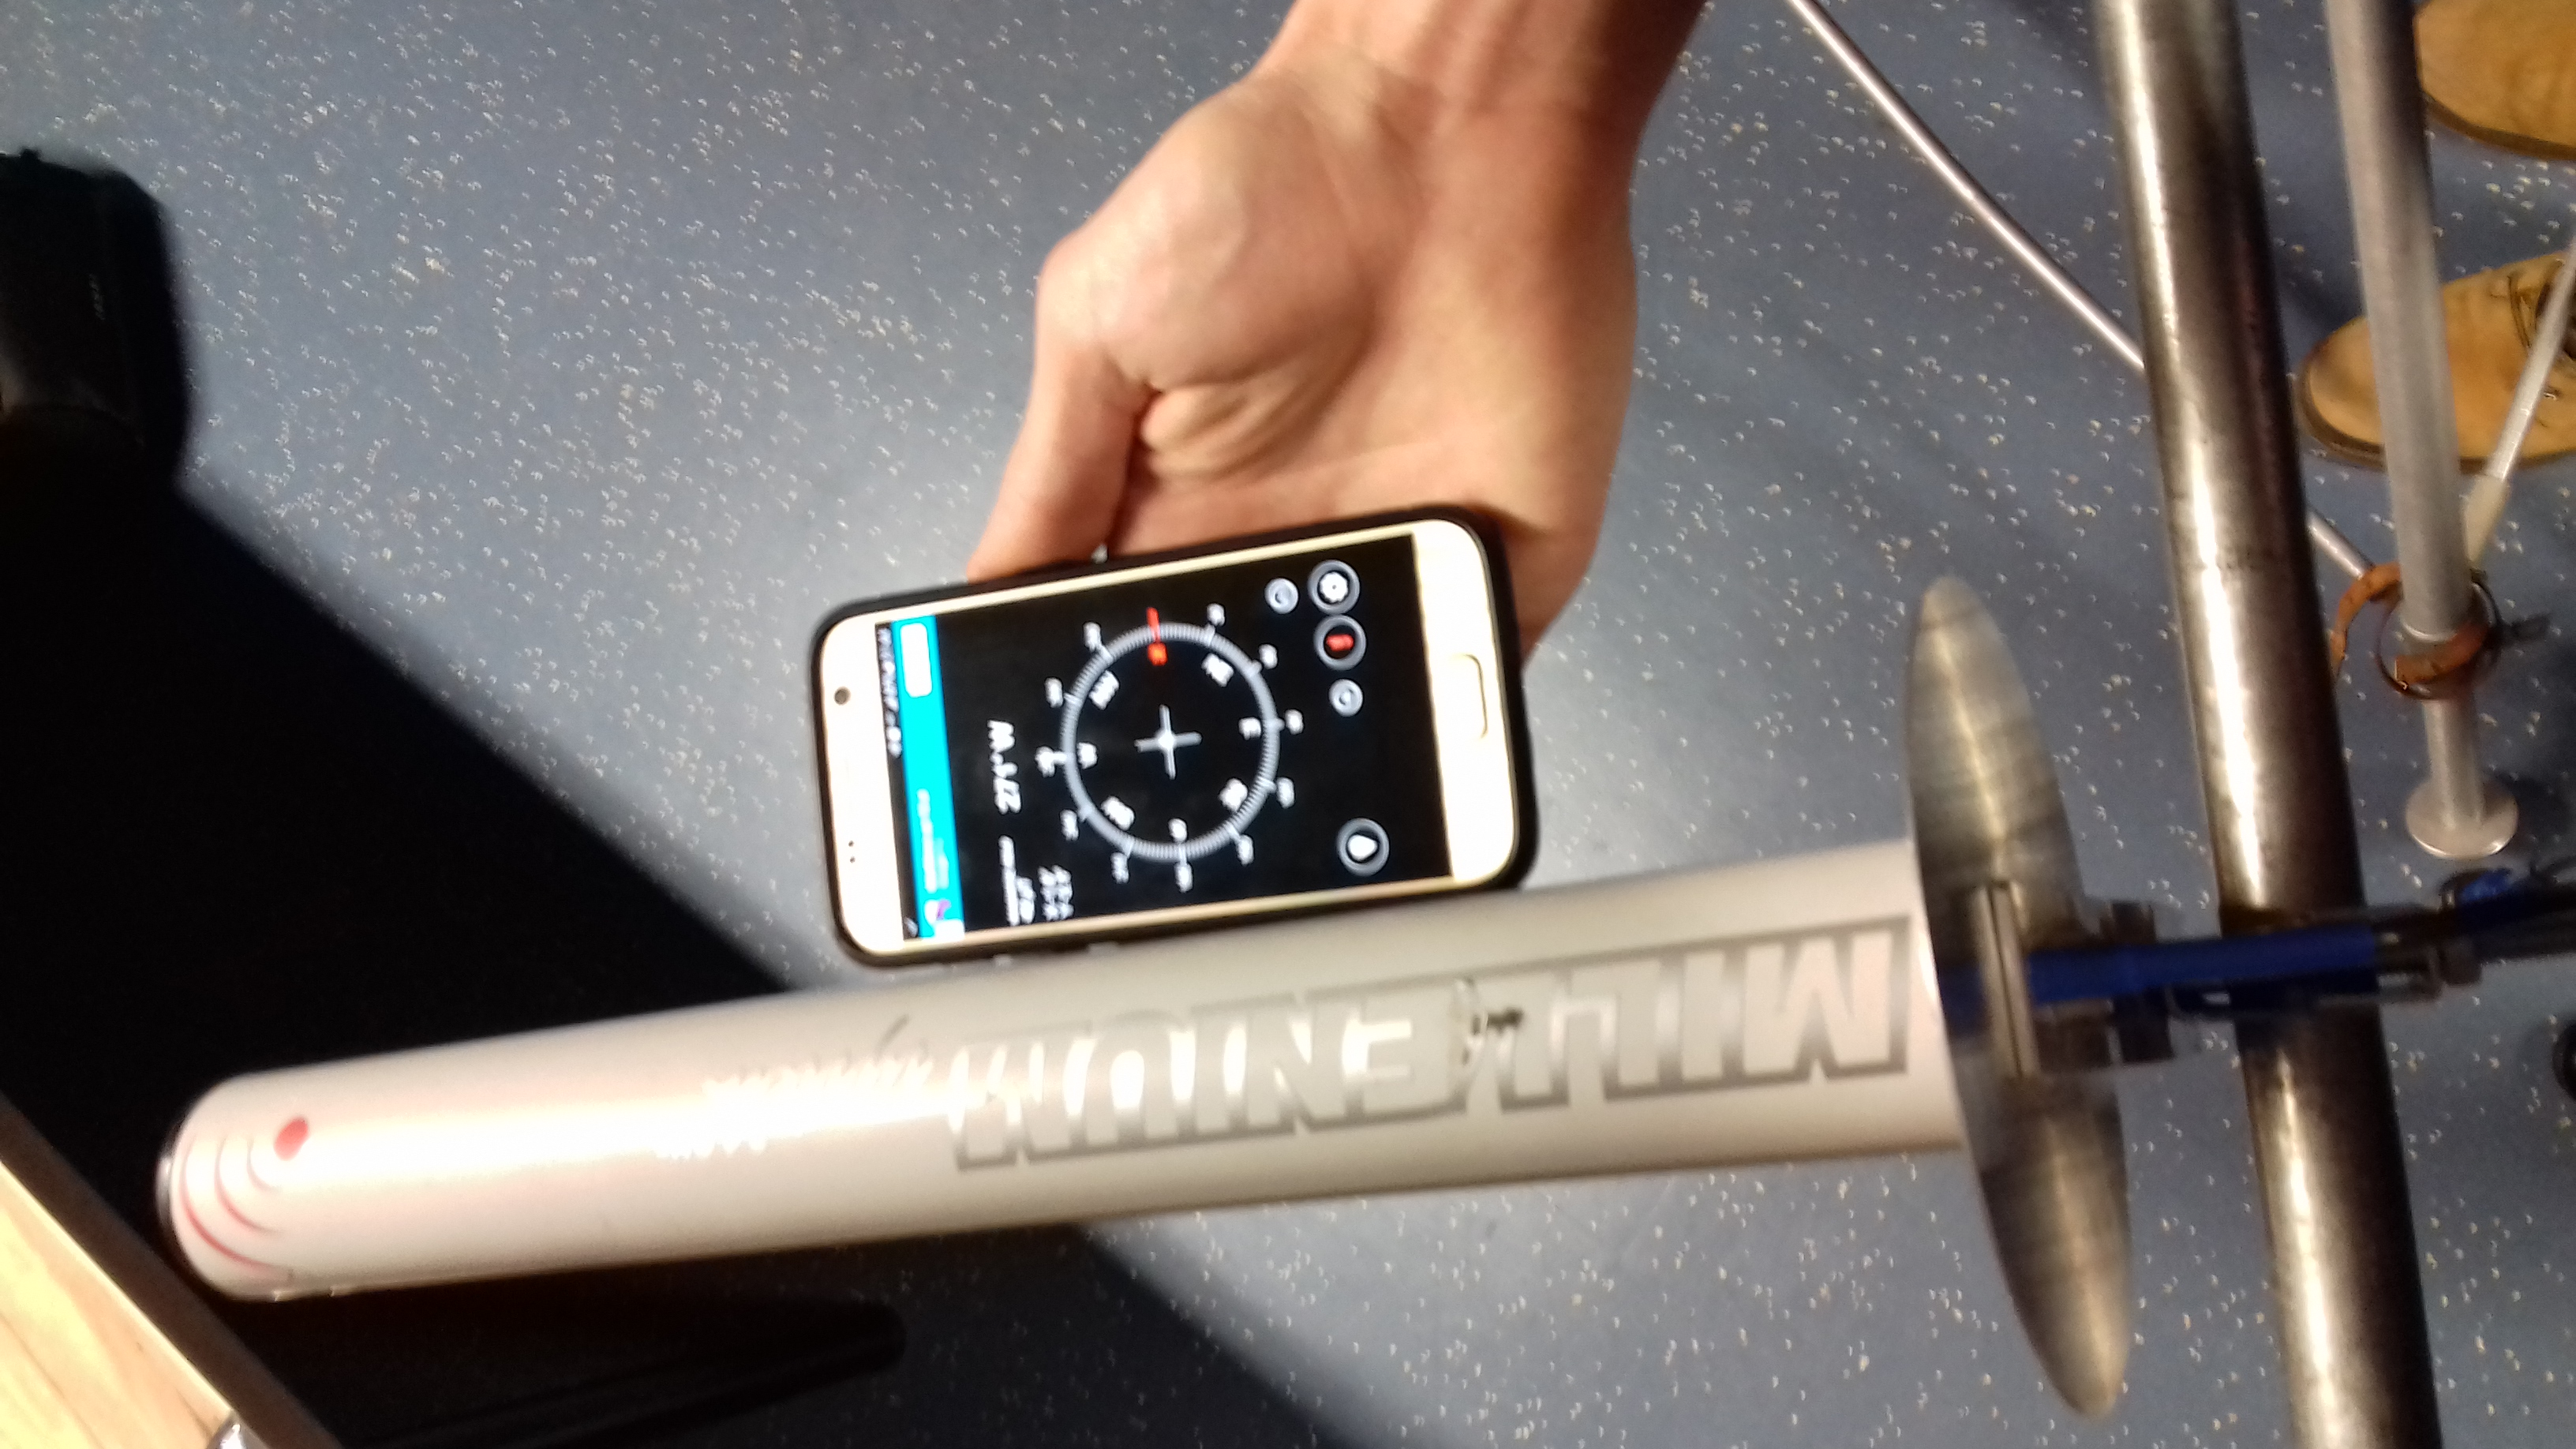
\includegraphics[width=\textwidth]{test_kierunku}
 \centering
 \caption{Sprawdzenie orientacji anteny przy pomocy zewnętrznego kompasu.}
 \label{kompas}
\end{figure}

% \todo{zjdecia w katalogu testy}

\subsection{Część radiowa}

Niemożliwe były testy bezpośrednie odbioru sygnału APRS ze względu na brak radia SDR na zadane pasmo częstotliwości, więc testy ograniczono do tych opisanych w poprzednim rozdziale.

\subsection{Podsumowanie}

Celem projektu było opracowanie mobilnej stacji do łączności radiowej z
balonem ze szczególnym zwróceniem uwagi na pasma radioamatorskie.
Stacja składa się z:
\begin{itemize}
 \item statywu z elektronicznie sterowanymi antenami,
 \item przy pomocy silników DC umożliwiających zmianę orientacji anten w płaszczyźnie azymutu i elewacji,
 \item radia programowalnego (SDR – Software
Defined Radio) do przetworzenia sygnału (wykorzystane zostało radio
będące na stanie Laboratorium Technologii Kosmicznych WEiTI),
 \item oprogramowanie SDR umożliwiające odbiór pakietów
APRS - automatycznego systemu powiadamiania o pozycji, który jest
zwykle wykorzystywany do lokalizacji balonów w misjach.
\end{itemize}

Opracowana stacja pozwalała na odbiór sygnałów w pasmach
radioamatorskich UHF (430 MHz) oraz VHF (140 MHz).
Opracowany rotor, obracający anteny w płaszczyźnie azymutu i elewacji,
może być zamontowany na rozkładanym statywie antenowym lub na
dachu samochodu (z wykorzystaniem bagażnika dachowego)

\input{podsumowanie}
\begin{thebibliography}{[1]}

\bibitem{dde}
http://tripsintech.com/orbitron-dde-azimuth-elevation-to-serial/

\end{thebibliography}


% \begin{thebibliography}{[1]}
% 
%  \bibitem{aprs}mgr. inż. Walczyk M., ``Opracowanie i badanie systemu miniAPRS dla misji balonowych'', praca dyplomowa magisterska Politechnika Warszawska 2013/14
% \end{thebibliography}



\label{ENDOFDOC}
\end{document}
